\section{Projektplanung}
\label{sec:chapterexample}

\subsection{Prozess}
\label{sec:chapterexample}
Als Entwicklungsprozess wird ein hybrides Vorgehensmodell eingesetzt, welcher in Abbildung \ref{fig:hybridesModell} dargestellt wird. Im Rahmen einer Bachelorarbeit, in der die Anforderungen und Analysen schon im voraus im Fachmodul definiert worden sind, eignet sich am bestens ein lineares V-Modell. Ein solcher Prozess ist sehr schlank, übersichtlich und für diese Projektgrösse geeignet.
\\
Was das V-Modell nicht erlaubt, ist eine ständige Iteration mit dem Kunden während der Entwurf/Implementierungsphase. Daraus ergibt sich, wie im Abbild unten gezeigt, ein hybrides Modell welches uns zulässt, trotz der klar definierten Anforderungen, während der Entwurf- und der Implementierungsphase ein agiles Vorgehen mit dem Kunden durchzuführen.
\\
Die im Fachmodul geleistete Arbeit gehört zu den ersten zwei Phasen des Modells. Wie im linearen Vorgehensmodell vorgegeben, beginnt die nächste Phase der Arbeit sobald die vorherige Phase abgeschlossen ist. Die ganze Bachelorarbeit basiert auf Evaluationen und Entscheidungen, die in den ersten Phasen des Projekts getroffen worden sind. 

\begin{figure}[htb!]
	\begin{center}
		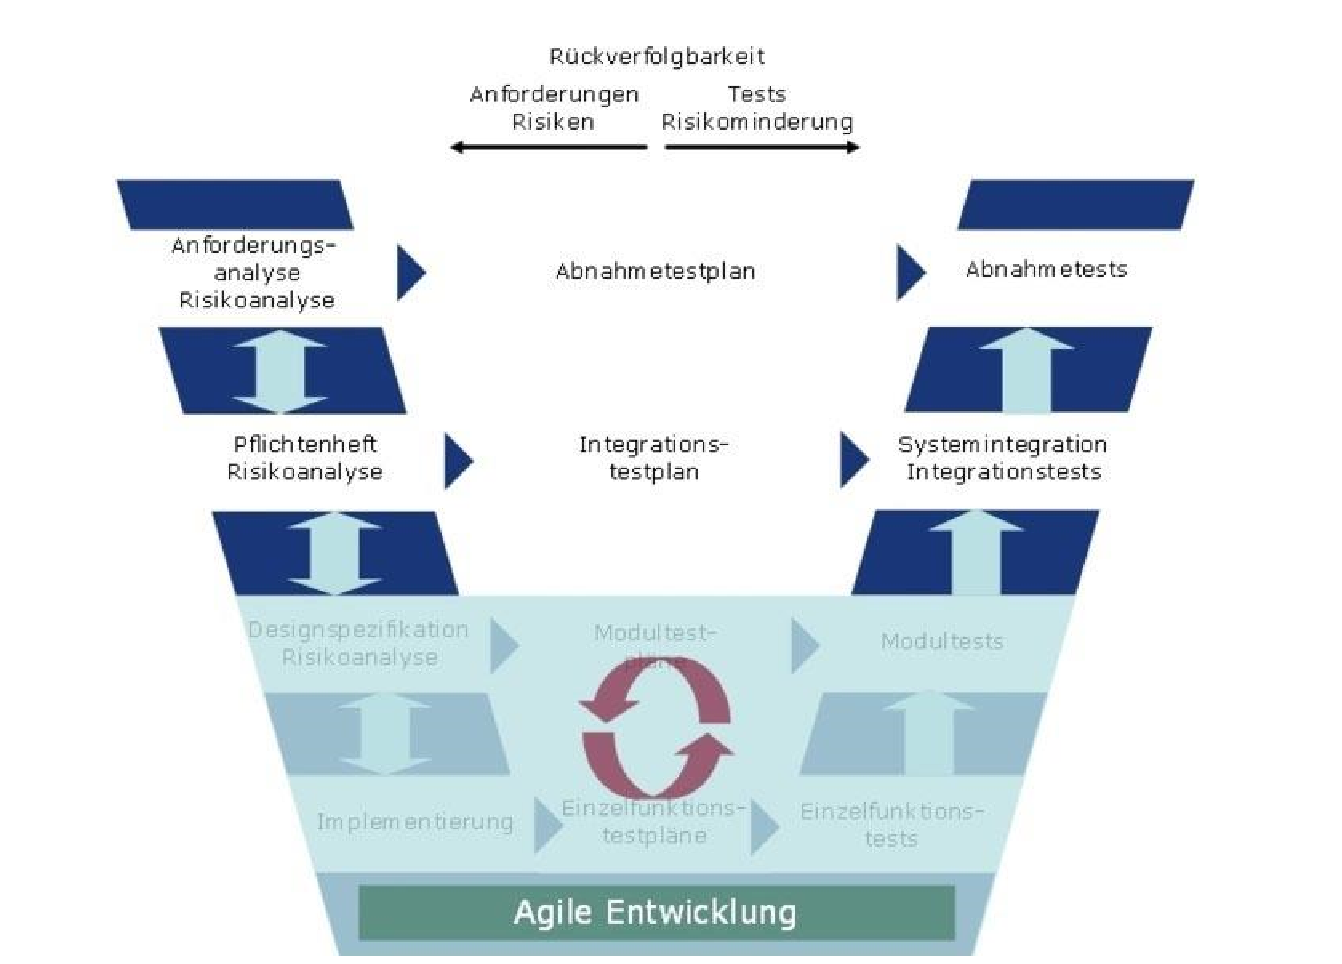
\includegraphics[width=0.89\textwidth]{hybridesModell}
		\caption[Hybrides Vorgehensmodell]{Hybrides Vorgehensmodell}
		\label{fig:hybridesModell}
	\end{center}
\end{figure}


\subsection{Zeitplanung}
\label{sec:zeitplanung}
Die folgenden Abbildungen stellen die Projektplanung und die Meilensteine zeitlich dar (\seeref{fig:projektPlanungAchse} \& \cref{fig:projektPlanung}). In die erste Woche werden die Hardwarekomponenten, die mittlerweile schon bestellt wurden, getestet und zusammengebaut. 
\\
Die nächste zwei Hauptpunkte betreffen die Programmierung der  Software, die in zwei Teile geteilt wurde.
\\ 
Beim Teil 1 geht es um die Skripts die serverseitig kleine Aufgaben übernehmen, beim Teil 2 geht es um die Programmierung der Software. Da werden die Webapplikationen entwickelt, die auf den Aussensprechstellen und auf den mobilen Geräten der Bewohner ausgeführt werden sollen.
\\
Die letzte Phase ist für die Optimierung und als Reserve gedacht.

\begin{figure}[htb!]
	\begin{center}
		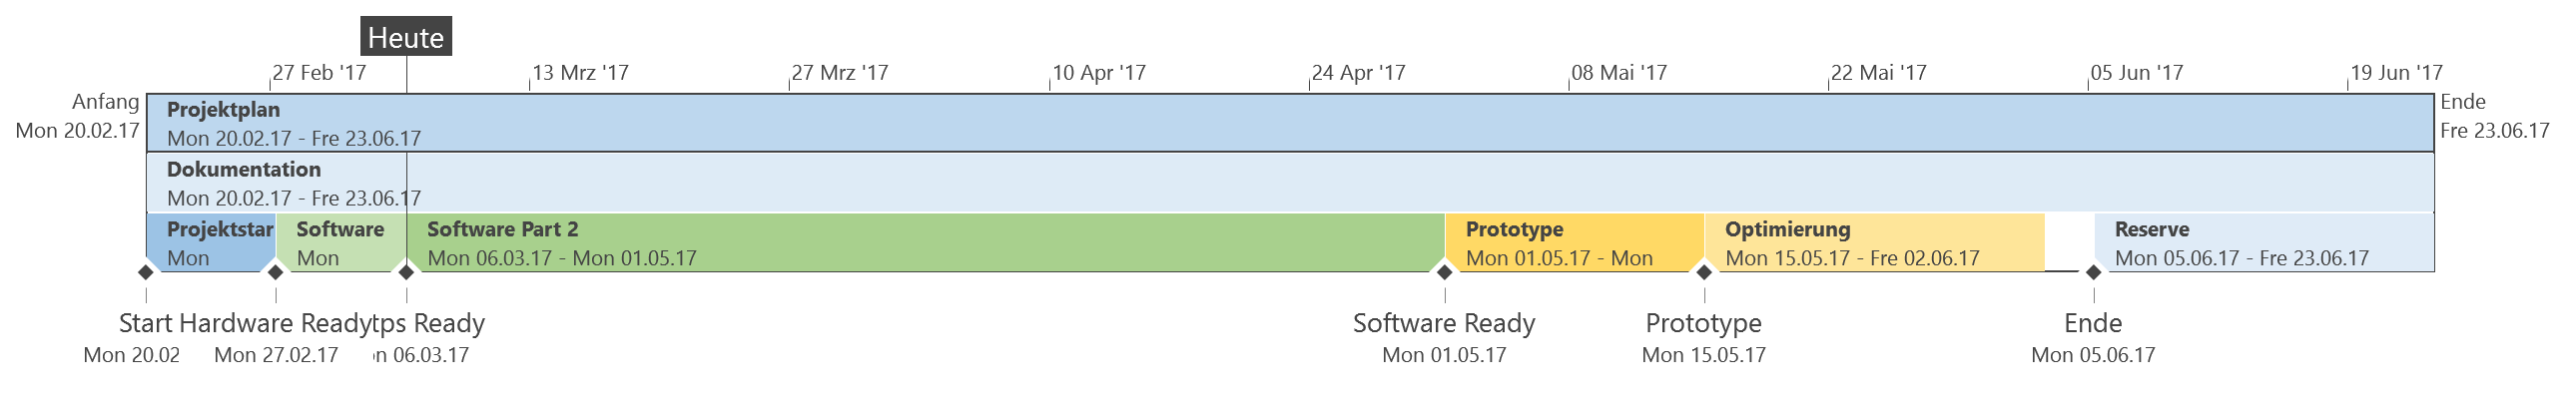
\includegraphics[width=1\textwidth]{projektPlanAchse}
		\caption[Projektplanung Meilensteine]{Zeitplanung mit Meilensteine}
		\label{fig:projektPlanungAchse}
	\end{center}
\end{figure}


\begin{figure}[htb!]
	\begin{center}
		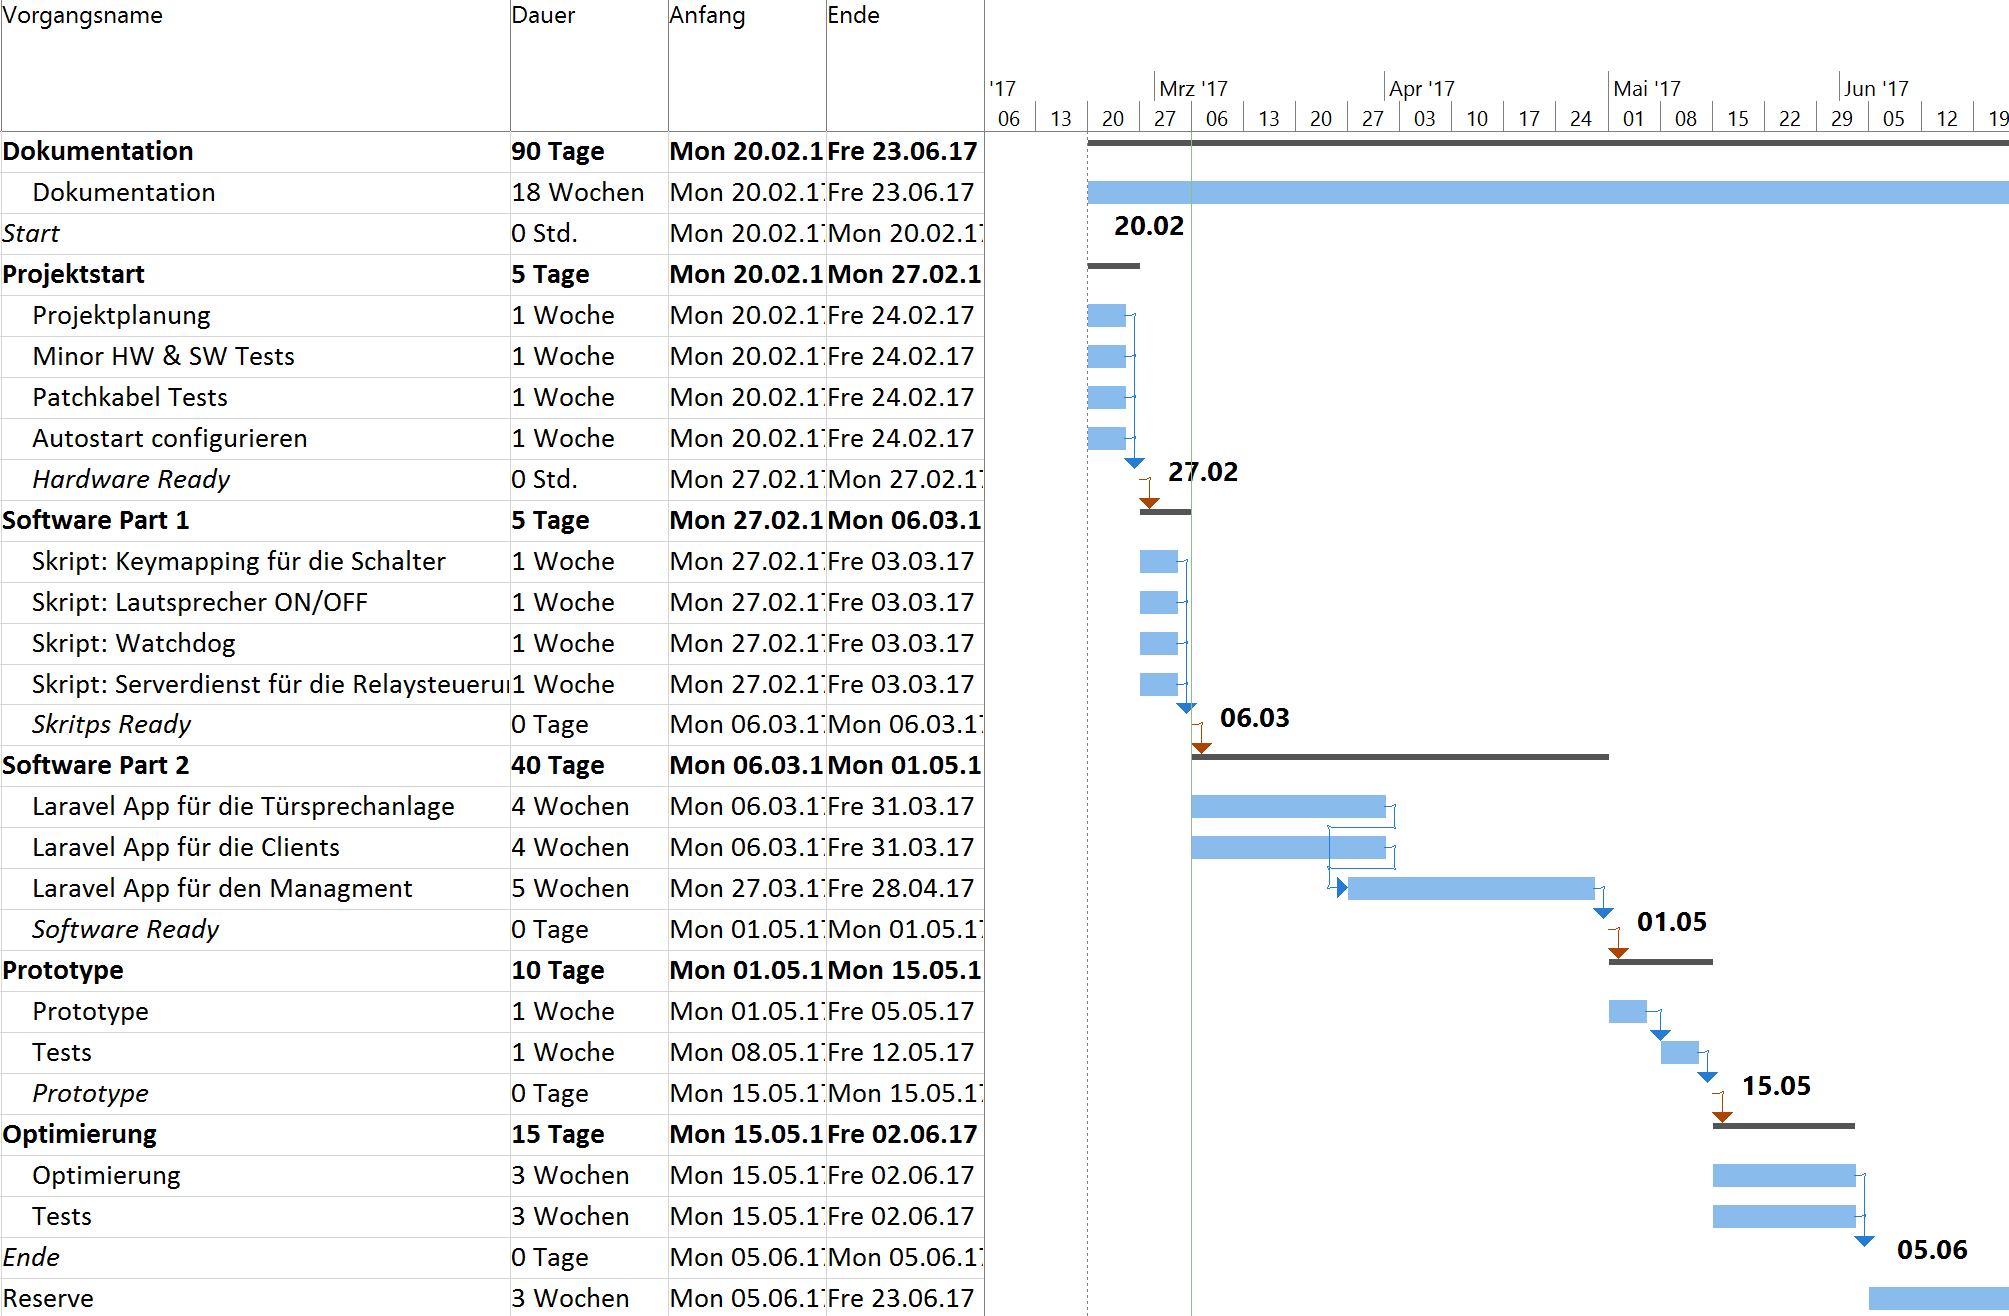
\includegraphics[width=0.9\textwidth]{projektPlanung}
		\caption[Projektplanung]{Projektplanung}
		\label{fig:projektPlanung}
	\end{center}
\end{figure}

\subsection{Versionierung}
Für die Versionierung und die gesamte Entwicklung wird das etablierte Open-Source Version-Control Software GIT verwendet. Das gesamte Quellcode, alle Bilder und Dokuemente werden in einem Repository gespeichert und versioniert.
\\
\\
Während die Entwicklung wird der Quellcode aber nicht Open-Source sein. Das Quellcode und die gesamte Entwicklungsdokumentation für das Projekt wird Vertraulich gehalten und nur für die Entwickler und Projektteilnehmer verfügbar sein. Für die Repository und das Backup wird also den Consumer Dienst Bitbucket verwendet.
\\
\\
Bitbucket (\seeref{fig:bitbucket})ist ein webbasierter Filehosting-Dienst für Software-Entwicklungsprojekte, der die Versionsverwaltungssystem e Git und Mercurial unterstüzt. Bitbucket ermöglicht auch die Zusammenarbeit von mehreren Benutzern am gleichen Projekt. Bitbucket ist für ein Projekt dieser grosse kostenfrei.
\begin{figure}[htb!]
	\begin{center}
		
\includegraphics[width=1\textwidth]{bitbucket}
		\caption[Bitbucket ist ein Filehosting und ein Dienst für die Versionskontrolle von Softwareprojekte]{Bitbucket ist ein Filehosting und ein Dienst für die Versionskontrolle von Softwareprojekte}
		\label{fig:bitbucket}
	\end{center}
\end{figure}
\newpage
